\documentclass[]{article}

% accenti
\usepackage[utf8]{inputenc}
% rimuove identatura
\usepackage[parfill]{parskip}
% colori
\usepackage{color}
\usepackage{vmargin}

\usepackage{graphicx}
\begin{document}

%\setpapersize{A4}
%\setmarginsrb{15mm}{10mm}{15mm}{10mm}
%            {0mm}{10mm}{0mm}{10mm}

\title{Tabelle hash}
\author{Federico Magnolfi}
\maketitle


\section{Obbiettivo}
L'obbiettivo è verificare come si comportano le \textbf{tabelle hash} al crescere del numero di dati inseriti all'interno di esse. 

\section{Analisi}
Una tabella hash è una struttura dati usata per gestire un insieme di elementi detti chiavi, eventualmente collegate ad un valore.

Si sfrutta il concetto di funzione hash, una funzione che ha come dominio l'insieme delle chiavi, e come codominio i primi m numeri interi \{0, 1, 2, ..., m-1\}

La dimensione m della tabella viene scelta in base al numero di chiavi che si pensa di gestire. Data una chiave, la sua posizione all'interno della tabella è determinata in tempo costante dalla funzione hash.
Essendo essa non iniettiva, chiavi diverse potrebbero determinare la stessa posizione all'interno della tabella: in questo caso si parla di collisione. Questo problema può essere risolto in più modi, si analizzano i seguenti:
\begin{itemize}
\item indirizzamento aperto con ispezione lineare: ogni elemento del vettore è una chiave oppure un valore speciale che indica uno spazio vuoto. Quando si vuole inserire una chiave, se la casella corrispondente risulta già occupata da un'altra chiave, si usa la casella successiva, al termine della tabella si ricomincia dall'inizio (analogo per la ricerca). Il fenomeno di addensamento di chiavi in slot contigui è detto cluster primario.
\item concatenamento: ogni elemento del vettore è una lista concatenata. L'inserimento di una chiave viene fatto nella lista di indice corrispondente (analogo per la ricerca).
\end{itemize}

Si definiscono:
\\n = numero di elementi contenuti nella tabella
\\$\alpha$ = n/m

Si vuole sperimentare come cambia il numero di collisioni che si hanno a seconda del metodo di gestione delle collisioni ed all'aumentare di n, fino ad arrivare ad $\alpha$ = 1.\\
Inoltre, per il metodo basato su indirizzamento aperto con ispezione lineare, si vuole misurare come variano la lunghezza media e massima dei blocchi di addensamento di chiavi (cluster/sequenze) in funzione di n.

Si considerano tabelle hash contenenti soltanto chiavi, in quanto l'eventuale valore associato non è utile per studiare il numero di collisioni e lunghezza dei cluster. Si considera come insieme delle chiavi l'insieme dei numeri interi. La funzione hash viene calcolata con il metodo delle divisioni: essa funziona bene quando il numero utilizzato per calcolare il modulo è un numero primo.

\subsection*{Aspettative}
Visto che la percentuale massima testata è il 100\%, si avrà sempre $n \leq m$
All'aumentare di n, nell'indirizzamento aperto aumenteranno sicuramente la lunghezza media e massima dei cluster, esse saranno massime quando le chiavi inserite occupano posti contigui: in questo caso (se $n < m$) la lunghezza massima è uguale ad n, quella media è uguale ad $n*(n+1)/(2m)$.

Inoltre ci si aspetta che  le collisioni aumentino per entrambe le implementazioni:
\begin{itemize}
\item per l'indirizzamento aperto, durante il singolo inserimento, ci saranno tante più collisioni quanto più lunga sarà la sequenza da scorrere: quindi il numero totale di collisioni crescerà molto velocemente sopra una certa soglia di caricamento. Nel caso peggiore, durante l'inserimento $i$-esimo (i=0, 1, ...) si avranno $i$ collisioni, quindi il massimo numero di collisioni sarà $m*(m-1)/2$.
\item per il concatenamento, ci sarà al massimo una collisione per ogni singolo inserimento: il numero totale di collisioni sarà minore o uguale ad $n$.
\end{itemize}

\section{Test}
Nel file \textit{hash.py} si implementano i due tipi di tabelle hash in Python:
\begin{itemize}
\item per l'indirizzamento aperto, la tabella contenente le chiavi è una lista contenente valori interi oppure \textit{None} quando la casella è vuota.
\item per il concatenamento, la tabella contenente le chiavi è una lista di liste.
\end{itemize}

Per entrambe le implementazioni, le operazioni permesse sono inserimento, ricerca e cancellazione.

La lunghezza della tabella desiderata può essere indicata specificando un parametro nel costruttore: visto che la funzione hash scelta funziona bene quando m è primo, se il parametro non è primo, m sarà il numero primo più vicino al parametro ($>$ per l'indirizzamento aperto, $<$ per il concatenamento).

Si eseguono i test con m = 1000, che diventa quindi 1009 per l'indirizzamento aperto e 997 per il concatenamento.
Il numero di inserimenti effettuati ad ogni test è una percentuale rispetto ad m, il valore di ogni numero inserito è generato casualmente tra $0$ e $100*m$.
Per ogni schema di gestione delle collisioni, si testano le percentuali: [10, 20, 30, 40, 50, 60, 70, 75, 80, 85, 87, 89, 90, 91, 92, 93, 94, 95, 95, 97, 98, 99, 100].

Nel file \textit{test.py}, per ogni percentuale si eseguono 20 test, i valori che vengono misurati sono:
\begin{itemize}
\item numero totale di collisioni per l'indirizzamento aperto: si misura il numero minimo, medio e massimo nell'arco dei 20 test
\item lunghezza delle sequenze per l'indirizzamento aperto: si misura il numero medio* e massimo nell'arco dei 20 test
\item numero totale di collisioni per il concatenamento: si misura il numero minimo, medio e massimo nell'arco dei 20 test
\end{itemize}

*: \textit{dopo aver effettuato tutti gli inserimenti, con lunghezza media della sequenza si intende la lunghezza attesa della sequenza da scorrere in un prossimo ipotetico inserimento. Si suppone che l'hash della chiave da inserire generi uno degli m indici con la stessa probabilità (hash uniforme semplice). Non si misura la minima lunghezza delle sequenze in quanto non si ritiene un dato significativo: essa sarebbe 0 se la tabella non è piena, altrimenti sarebbe la lunghezza della tabella quando è piena. Quando la tabella è piena, per una migliore visualizzazione grafica si considera la lunghezza di ogni sequenza pari ad m, anche se in teoria si potrebbe considerare una lunghezza infinita.}

Viene lanciato il programma \textit{exp.py}, che scrive sul file "testInput.p" i test da effettuare e richiama la funzione di test, che scrive i risultati nel file "testOutput.p". Per la lettura e la scrittura di oggetti su file, si usa il modulo pickle.

L'input dei test è un oggetto del seguente tipo: lista con due elementi, il primo è m, mentre il secondo è la lista di percentuali da testare.

L'output dei test viene caricato in un dizionario che sarà formato nel seguente modo:
\begin{verbatim}
{
percentuale1:
    [minColIA, medColIA, maxColIA, medSeqIA, maxSeqIA, minColC, medColC, maxColC],
percentuale2: [...],
...
}
\end{verbatim}
Viene eseguita una stampa su console del dizionario per visualizzare i dati numerici ottenuti.

Utilizzando il modulo matplotlib.pyplot, si interpretano i dati contenuti nel dizionario per realizzare tre grafici, in modo da rendere l'idea dell'andamento delle misure.

\section{Risultati}
I dati ottenuti dai test sono i seguenti:
\begin{verbatim}
{
10: [2, 4.6, 8, 0.1, 5, 2, 4.8, 9],
20: [18, 24.8, 36, 0.3, 10, 10, 17.6, 24],
30: [44, 62.5, 90, 0.5, 11, 29, 41.0, 51],
40: [90, 128.8, 163, 0.9, 18, 58, 70.0, 84],
50: [223, 250.8, 297, 1.5, 24, 93, 107.3, 124],
60: [376, 465.6, 644, 2.6, 35, 133, 145.7, 160],
70: [603, 790.1, 997, 4.8, 69, 183, 196.8, 214],
75: [793, 1100.7, 1408, 6.9, 102, 203, 221.4, 244],
80: [1047, 1534.0, 2205, 11.1, 149, 233, 249.4, 270],
85: [1836, 2383.3, 3408, 20.5, 273, 264, 275.9, 293],
87: [1762, 2915.8, 4727, 26.5, 281, 278, 287.5, 305],
89: [2177, 3443.4, 4712, 35.7, 306, 281, 297.1, 321],
90: [2393, 3625.1, 5549, 38.8, 338, 291, 307.1, 327],
91: [2476, 4015.9, 6560, 50.9, 496, 297, 312.3, 335],
92: [3098, 4593.1, 7192, 54.9, 500, 301, 315.5, 340],
93: [2932, 4857.8, 6424, 65.5, 543, 309, 322.8, 343],
94: [3773, 5715.4, 8096, 91.0, 649, 314, 329.9, 341],
95: [3283, 7365.1, 13799, 104.0, 601, 309, 332.2, 357],
97: [7391, 9941.5, 14570, 185.6, 891, 333, 349.5, 369],
98: [5546, 11969.7, 22669, 230.7, 929, 339, 354.6, 372],
99: [7250, 14665.3, 24532, 333.1, 987, 344, 360.7, 378],
100: [10001, 20978.3, 34457, 1009.0, 1009, 358, 369.6, 382]
}
\end{verbatim}

Vengono quindi creati i 3 grafici nel seguente modo:
\begin{itemize}
\item numero totale di collisioni per l'indirizzamento aperto: tre funzioni che indicano il numero minimo, medio e massimo nell'arco dei 20 test, i punti delle funzioni hanno la percentuale come ascissa, le corrispondenti ordinate sono i primi tre elementi della lista associata alla percentuale.
\item lunghezza delle sequenze per l'indirizzamento aperto: due funzioni che indicano il numero medio e massimo nell'arco dei 20 test, i punti delle funzioni hanno la percentuale come ascissa, le corrispondenti ordinate sono il quarto e il quinto elemento della lista associata alla percentuale.
\item numero totale di collisioni per il concatenamento: tre funzioni che indicano il numero minimo, medio e massimo nell'arco dei 20 test, i punti delle funzioni hanno la percentuale come ascissa, le corrispondenti ordinate sono gli ultimi tre elementi della lista associata alla percentuale.
\end{itemize}

\subsection*{Collisioni in indirizzamento aperto}
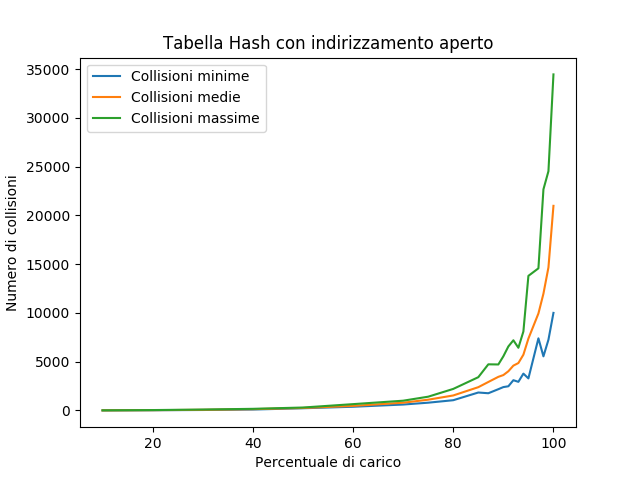
\includegraphics {IA-collisioni.png}
Nelle tabelle ad indirizzamento aperto il numero di collisioni cresce all'incirca in modo lineare fino al 70-80\%, dopodiché assume un andamento esponenziale.

\subsection*{Lunghezza sequenze in indirizzamento aperto}
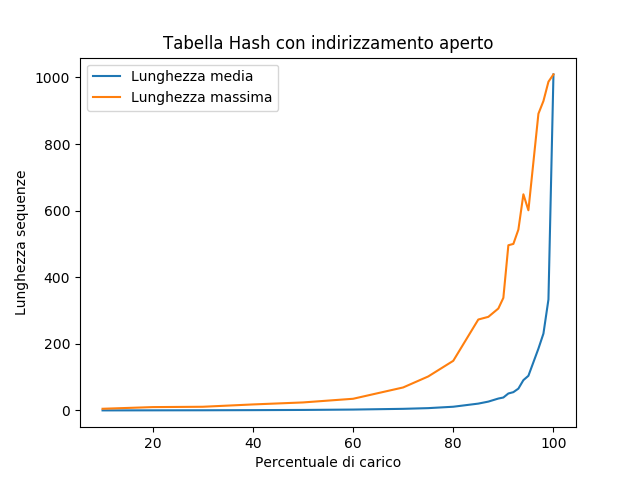
\includegraphics {IA-sequenze.png}
Nelle tabelle ad indirizzamento aperto la lunghezza delle sequenze cresce all'incirca in modo lineare fino al 60\%, dopodiché assume un andamento esponenziale.

\subsection*{Collisioni in concatenamento}
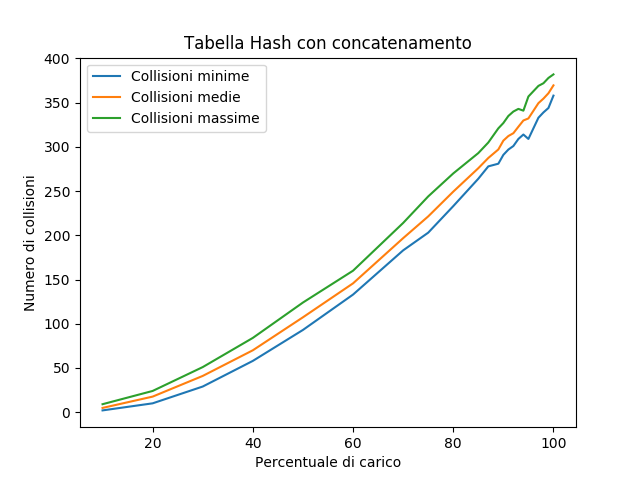
\includegraphics {C-collisioni.png}
Nelle tabelle con concatenamento, il numero di collisioni cresce all'incirca in modo lineare.

\section{Conclusione}
Nell'indirizzamento aperto, il numero di collisioni e la lunghezza delle sequenze inizia ad aumentare esponenzialmente intorno alla soglia del 70\%: superata questa percentuale di caricamento, la cosa migliore da fare sarà creare una nuova tabella con un m decisamente più grande, per evitare un aumento eccessivo del tempo di esecuzione delle operazioni di inserimento, ricerca e cancellazione.

Nel concatenamento, il numero di collisioni è all'incirca lineare: questo tipo di implementazione è quindi preferibile se si pensa di effettuare in prevalenza operazioni di inserimento.

I dati misurati sono coerenti con le aspettative.



\end{document}